\documentclass[11pt]{article}
\usepackage[utf8]{inputenc}
\usepackage[T1]{fontenc}
\usepackage[spanish,es-noshorthands]{babel}
\usepackage[margin=2.5cm]{geometry}
\usepackage{amsmath,amssymb}
\usepackage{graphicx}
\usepackage{booktabs}
\usepackage{xcolor}
\usepackage[colorlinks=true,linkcolor=blue,citecolor=blue]{hyperref}
\usepackage{caption}
\usepackage{parskip}
\usepackage[expansion=false]{microtype}
\sloppy

\title{\textbf{$\beta$ por capa vs. $\beta$ global en un crossbar\\
con capa oculta de 100 neuronas (ReLU)}}
\author{Walter Quiñonez}
\date{Reporte generado con Claude Code \textperiodcentered\ 13 de septiembre de 2026}

\begin{document}
\maketitle

\begin{quote}\itshape
Exploración pedida en \texttt{prompt.txt}: para una arquitectura
\texttt{[784, 100, 10]} (capa oculta de 100 neuronas con ReLU, capa de
salida lineal), ¿conviene usar un $\beta$ distinto para la capa oculta y la
de salida, o alcanza con un único $\beta$ global? Se mapeó el accuracy en
una grilla log-espaciada de $(\beta_{oculta}, \beta_{salida})$, para una
curva P/D lineal y una no lineal, con el protocolo mínimo validado en
\texttt{analisis\_epochs\_series\_minimos/} ($k$=3 folds, 8 épocas,
\emph{common random numbers} entre puntos de la grilla). No se modificó
ningún código existente del proyecto.
\end{quote}

\tableofcontents


\section{Resumen ejecutivo}

\begin{table}[htbp]\centering

\begin{tabular}{@{}lrrr@{}}\toprule

Curva P/D & mejor acc. (beta único) & mejor acc. (beta por capa) & ganancia [pp] \\ \midrule

Curva P/D lineal (a=4567.9) & 95.23\% ($\beta$=338) & 95.32\% ($\beta_o$=134, $\beta_s$=536) & 0.09 \\

Curva P/D no lineal (a=98.55) & 91.63\% ($\beta$=121) & 92.49\% ($\beta_o$=121, $\beta_s$=305) & 0.87 \\

\bottomrule\end{tabular}

\caption{Comparación entre el mejor punto sobre la diagonal ($\beta_{oculta}=\beta_{salida}$, equivalente a un único $\beta$ global) y el mejor punto de toda la grilla ($\beta$ por capa libre).}

\end{table}

\section{Curva: Curva P/D lineal (a=4567.9)}

\begin{figure}[htbp]\centering

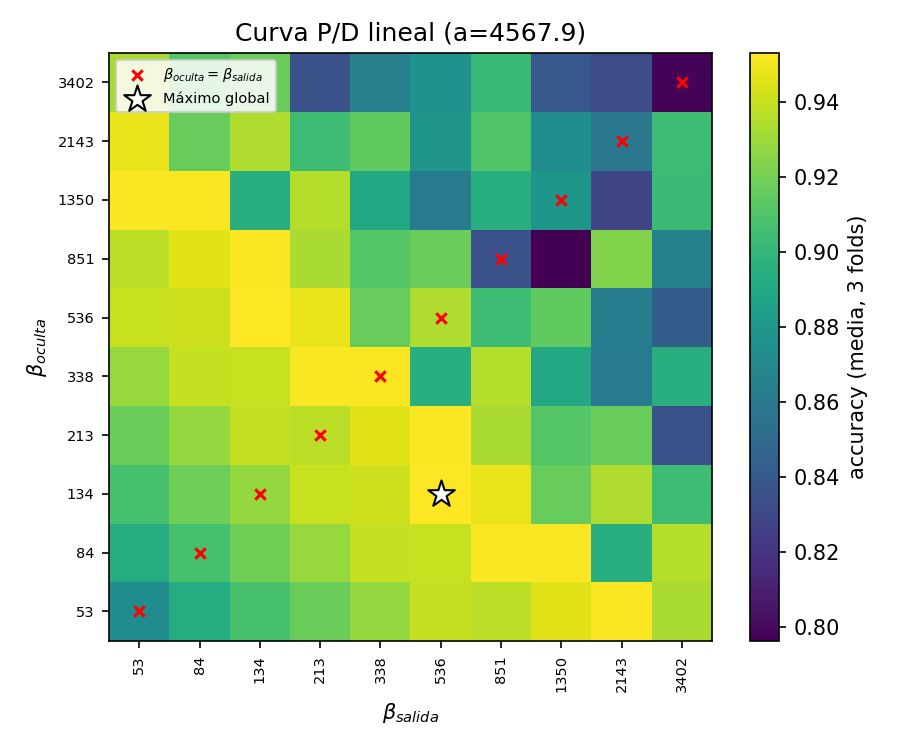
\includegraphics[width=0.75\textwidth]{heatmap_lineal.png}

\caption{Accuracy medio (3 folds) en función de $(\beta_{oculta}, \beta_{salida})$, Curva P/D lineal (a=4567.9). La cruz roja marca la diagonal (beta único); la estrella blanca, el máximo global.}

\end{figure}

Mejor punto sobre la diagonal (beta único global): $\beta$=337.6, acc=95.23\% (SEM 0.35pp).\\

Mejor punto global (beta por capa libre): $\beta_{oculta}$=134.0, $\beta_{salida}$=535.8, acc=95.32\% (SEM 0.22pp).\\

Ganancia del mejor beta-por-capa sobre el mejor beta-único: \textbf{0.09 puntos porcentuales}.

\section{Curva: Curva P/D no lineal (a=98.55)}

\begin{figure}[htbp]\centering

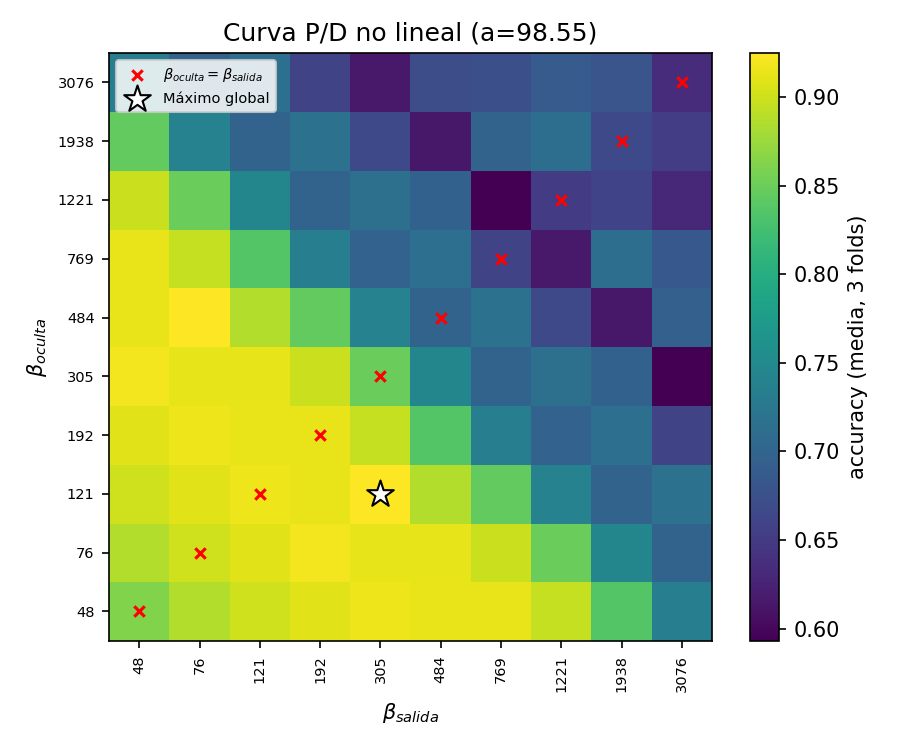
\includegraphics[width=0.75\textwidth]{heatmap_no_lineal.png}

\caption{Accuracy medio (3 folds) en función de $(\beta_{oculta}, \beta_{salida})$, Curva P/D no lineal (a=98.55). La cruz roja marca la diagonal (beta único); la estrella blanca, el máximo global.}

\end{figure}

Mejor punto sobre la diagonal (beta único global): $\beta$=121.1, acc=91.63\% (SEM 0.22pp).\\

Mejor punto global (beta por capa libre): $\beta_{oculta}$=121.1, $\beta_{salida}$=305.2, acc=92.49\% (SEM 0.22pp).\\

Ganancia del mejor beta-por-capa sobre el mejor beta-único: \textbf{0.87 puntos porcentuales}.

\section{Por qué la grilla es (casi) simétrica en el producto $\beta_{oculta}\cdot\beta_{salida}$}

En los heatmaps de las Secciones 2 y 3 se observa que puntos muy alejados de la diagonal (splits muy desparejos entre las 2 capas) pueden dar el mismo accuracy que un punto cercano a la diagonal, siempre que el \emph{producto} $\beta_{oculta}\cdot\beta_{salida}$ sea parecido. Esto no es casualidad: tiene una razón matemática exacta.

El forward pass de este modelo (\texttt{MemDNN.forward}, sin bias) es $h=\mathrm{ReLU}(\beta_{oculta}\,(x W_1))$, $\mathrm{logits}=\beta_{salida}\,(h W_2)$. La ReLU es homogénea de grado 1 para escalares positivos: $\mathrm{ReLU}(c\,z)=c\,\mathrm{ReLU}(z)$ para todo $c>0$. Por lo tanto, para cualquier $c>0$, reemplazar $(\beta_{oculta},\beta_{salida}) \to (c\,\beta_{oculta},\, \beta_{salida}/c)$ deja \textbf{exactamente} el mismo $h$ escalado por $c$ y el mismo logit final (el $c$ se cancela): $h'=c\,h$, $\mathrm{logits}'=(\beta_{salida}/c)(c\,h\,W_2)=\mathrm{logits}$. Como la regla de actualización física de este proyecto (\texttt{Nmanhattan\_vectorizado}) sólo usa el \emph{signo} del gradiente para decidir potenciación/depresión (nunca su magnitud), y ese signo se deriva de los logits/softmax —que son idénticos bajo el reemplazo anterior—, la trayectoria completa de entrenamiento (qué pulso se aplica en cada paso) debería depender, en aritmética exacta, \textbf{sólo del producto $\beta_{oculta}\cdot\beta_{salida}$, no de cómo se reparte entre las 2 capas}.

\subsection{Verificación empírica: ¿la invariancia se sostiene en la práctica?}

Se corrieron splits muy distintos con el producto fijado en $\beta_{pred}^2$ de cada curva (fuera de la grilla 10$\times$10 principal, para no reciclar los mismos resultados):

\begin{table}[htbp]\centering\begin{tabular}{@{}lrrrr@{}}\toprule

Curva & $\beta_{oculta}$ & $\beta_{salida}$ & producto & accuracy (SEM) \\ \midrule

lineal & 425.29 & 425.29 & 180871.6 & 94.56\% (0.21pp) \\

lineal & 50.00 & 3617.43 & 180871.6 & 92.70\% (1.36pp) \\

lineal & 100.00 & 1808.72 & 180871.6 & 92.70\% (1.36pp) \\

lineal & 2000.00 & 90.44 & 180871.6 & 92.03\% (1.59pp) \\

no\_lineal & 384.52 & 384.52 & 147855.6 & 74.20\% (2.67pp) \\

no\_lineal & 2000.00 & 73.93 & 147855.6 & 72.97\% (2.10pp) \\

no\_lineal & 50.00 & 2957.11 & 147855.6 & 74.02\% (2.83pp) \\

no\_lineal & 100.00 & 1478.56 & 147855.6 & 74.02\% (2.83pp) \\

\bottomrule\end{tabular}

\caption{Splits muy distintos con el mismo producto $\beta_{oculta}\cdot\beta_{salida}$. Los pares (50, prod/50) y (100, prod/100) dan accuracy \emph{idéntico} (hasta el 6.º decimal, SEM incluido) en ambas curvas; el split ``natural'' ($\beta_{oculta}=\beta_{salida}=\sqrt{\text{prod}}$) y el split extremo (2000, prod/2000) difieren de esos hasta $\sim$2.5pp.}

\end{table}

Estas diferencias de hasta $\sim$2.5pp son del mismo orden que el propio SEM de la medición (hasta 2.83pp con sólo 3 folds), así que \textbf{no hay evidencia concluyente de que la invariancia se rompa de forma sistemática} más allá del ruido estadístico normal del protocolo mínimo usado. Es plausible que la causa de que algunos pares SÍ coincidan exactamente y otros no sea la naturaleza discreta de la actualización física (Manhattan, basada en el signo del gradiente): pequeñas diferencias de redondeo en float32 al computar $c\cdot\beta_{oculta}\cdot(xW_1)$ para $c$ muy distintos podrían, en principio, voltear el signo de algún pulso cerca de un umbral y desviar la trayectoria — pero con sólo 8 épocas y 3 folds esta hipótesis no se puede distinguir del ruido de muestreo con este experimento.

\section{Extensión analítica: ¿vale lo mismo con tangente hiperbólica?}

Todo lo anterior depende de una propiedad muy específica de la ReLU: ser homogénea de grado 1 ($\mathrm{ReLU}(cz)=c\,\mathrm{ReLU}(z)$ para $c>0$). La tangente hiperbólica NO tiene esa propiedad, así que vale la pena rehacer la cuenta para $h=\tanh(\beta_{oculta}(xW_1))$ en vez de $h=\mathrm{ReLU}(\beta_{oculta}(xW_1))$, manteniendo $\mathrm{logits}=\beta_{salida}(hW_2)$ y sin bias, igual que antes. \textbf{Esta sección es puramente analítica: no se corrió ninguna simulación nueva con tanh}, sólo se repite el argumento matemático de la Sección 4 para ver si sigue valiendo.

\subsection{La reparametrización $(\beta_{oculta},\beta_{salida})\to(c\,\beta_{oculta},\beta_{salida}/c)$ ya no es exacta}

Sea $z_1=\beta_{oculta}(xW_1)$ (pre-activación de la capa oculta). Con ReLU, escalar $\beta_{oculta}\to c\,\beta_{oculta}$ escala $z_1\to c\,z_1$ y, por homogeneidad, $h\to c\,h$ exactamente — ese factor $c$ se cancela después al dividir $\beta_{salida}$ por $c$. Con tanh, en cambio:

$$h' = \tanh(c\,z_1) \quad\text{mientras que}\quad c\cdot\tanh(z_1) = c\cdot h,$$

y en general $\tanh(cz)\neq c\,\tanh(z)$ para $c\neq 1$ (la única función homogénea de grado 1 y acotada es la nula). Por lo tanto $\mathrm{logits}' = (\beta_{salida}/c)\,\tanh(c z_1)\,W_2 \neq \beta_{salida}\,\tanh(z_1)\,W_2 = \mathrm{logits}$ salvo en el caso trivial $c=1$: \textbf{la invariancia exacta de la Sección 4 no se sostiene con tanh}. Con tanh, el resultado de la red depende en general de $\beta_{oculta}$ y $\beta_{salida}$ por separado, no sólo de su producto.

\subsection{Dos regímenes límite}

El tamaño del error de la aproximación se entiende mejor mirando los dos extremos de $z_1=\beta_{oculta}(xW_1)$:

\begin{itemize}

\item \textbf{$\beta_{oculta}$ chico (régimen lineal, $|z_1|\ll 1$):} usando $\tanh(z)=z-\tfrac{z^3}{3}+O(z^5)$,

$$\frac{\tanh(cz_1)}{c} = z_1 - \frac{c^2 z_1^3}{3} + O(z_1^5) \approx \tanh(z_1) - \frac{(c^2-1)}{3}z_1^3,$$

es decir, la invariancia exacta de ReLU se recupera de forma \emph{aproximada}, con un error relativo de orden $|c^2-1|\,z_1^2/3$: chico si $z_1$ es chico o si $c\approx 1$ (cerca de la diagonal), y creciente a medida que $\beta_{oculta}$ empuja $z_1$ lejos de 0. Esto es consistente con que la ReLU y la tanh son parecidas cerca del origen ($\tanh(z)\approx z\approx\mathrm{ReLU}(z)$ para $z>0$ chico).

\item \textbf{$\beta_{oculta}$ grande (régimen saturado, $|z_1|\gg 1$):} $\tanh(z_1)\to\mathrm{sign}(z_1)\in\{-1,+1\}$, una función de grado \emph{0} (no de grado 1): al seguir aumentando $\beta_{oculta}$, $h$ deja de crecer y se estanca en $\pm 1$ salvo muy cerca del borde de decisión $xW_1=0$. En este régimen $\beta_{oculta}$ ya no actúa como una ganancia multiplicativa de $h$ (como en ReLU), sino como un \emph{umbral/nitidez} de la frontera de decisión de cada neurona oculta, mientras que $\beta_{salida}$ sigue siendo la única ganancia lineal de los logits. Son dos roles cualitativamente distintos y, por construcción, ya no intercambiables vía ningún $c$.

\end{itemize}

\subsection{Conclusión analítica}

A diferencia de ReLU, con tanh en la capa oculta \textbf{no hay razón matemática para esperar que un único $\beta$ global sea tan bueno como optimizar $\beta_{oculta}$ y $\beta_{salida}$ por separado}. La aproximación por producto sigue siendo razonable sólo mientras $\beta_{oculta}$ mantenga la capa oculta en su tramo aproximadamente lineal ($|z_1|\lesssim 1$); apenas $\beta_{oculta}$ crece lo suficiente para saturar la tanh, el argumento se rompe cualitativamente y $\beta_{oculta}$ pasa a controlar algo distinto (la nitidez del umbral de cada neurona) de lo que controla $\beta_{salida}$ (la ganancia de los logits). Esto sugiere que, si se repitiera el experimento numérico de las Secciones 2--3 con tanh en vez de ReLU, sería esperable ver una ganancia real (no sólo ruido estadístico) de usar $\beta$ por capa, sobre todo en la zona de la grilla donde $\beta_{oculta}$ es grande — algo que este reporte no verifica numéricamente, sólo lo predice a partir de la forma funcional de la tanh.

\section{Verificación numérica con tanh}

Se repitió \textbf{exactamente} el experimento de las Secciones 2--3 (mismas curvas P/D, misma grilla log 10$\times$10, mismo protocolo mínimo, mismas semillas) reemplazando \texttt{MemDNN} por \texttt{MemDNNTanh} (subclase nueva en \texttt{mem\_dnn\_tanh.py} que sólo cambia \texttt{ReLU}$\to$\texttt{tanh} en la capa oculta; no se modificó \texttt{MemCrossbarClass\_beta\_por\_capa.py}).

\subsection{Grilla completa: diagonal vs. máximo global}

\begin{table}[htbp]\centering\begin{tabular}{@{}lrrr@{}}\toprule

Curva P/D & mejor acc. (beta único) & mejor acc. (beta por capa) & ganancia [pp] \\ \midrule

Curva P/D lineal (a=4567.9) & 95.07\% ($\beta$=338) & 95.13\% ($\beta_o$=536, $\beta_s$=338) & 0.06 \\

Curva P/D no lineal (a=98.55) & 92.36\% ($\beta$=192) & 93.03\% ($\beta_o$=1221, $\beta_s$=192) & 0.67 \\

\bottomrule\end{tabular}

\caption{Con tanh, misma comparación que el Cuadro 1 (ReLU).}

\end{table}

A primera vista esta ``ganancia'' (0.06pp lineal, 0.67pp no lineal) es \textbf{parecida o incluso menor} que la de ReLU (0.09pp y 0.87pp) — contrario a lo que predice la Sección 5. Esto es un artefacto de comparar sólo 2 puntos (el mejor de la diagonal y el mejor de toda la grilla): si el óptimo verdadero ya cae cerca de la diagonal para ambas activaciones, esa comparación puntual no alcanza a ver cuánto varía el accuracy con el split \emph{a igual producto}. La Sección 6.2 hace esa prueba directamente.

\begin{figure}[htbp]\centering

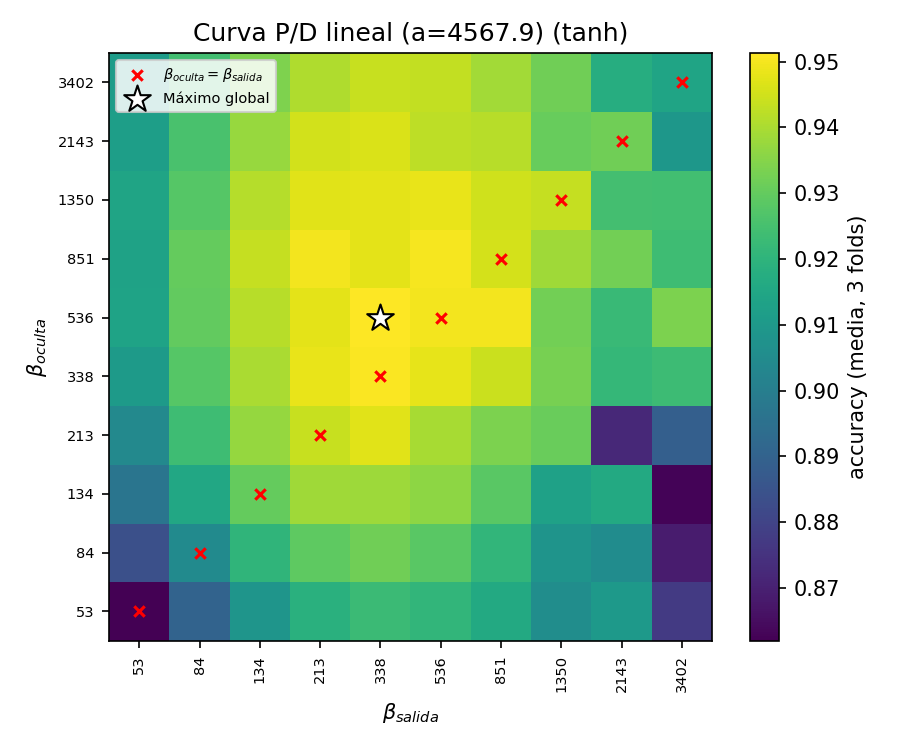
\includegraphics[width=0.7\textwidth]{heatmap_lineal_tanh.png}

\caption{Accuracy medio (3 folds) con tanh en la capa oculta, Curva P/D lineal (a=4567.9).}

\end{figure}

\begin{figure}[htbp]\centering

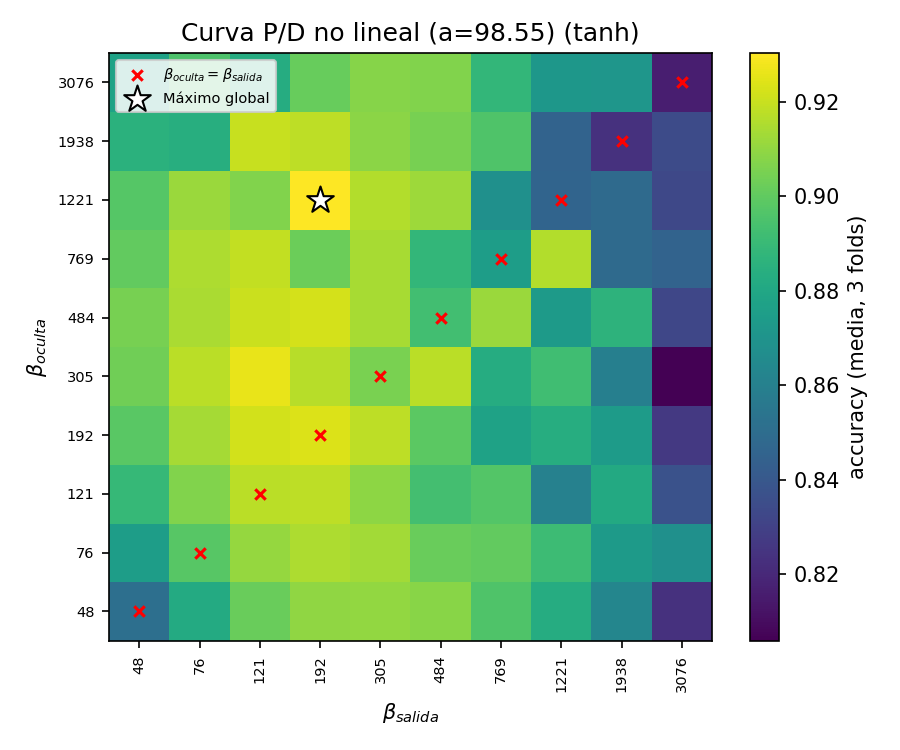
\includegraphics[width=0.7\textwidth]{heatmap_no_lineal_tanh.png}

\caption{Accuracy medio (3 folds) con tanh en la capa oculta, Curva P/D no lineal (a=98.55).}

\end{figure}

\subsection{Prueba directa: mismo producto, splits muy distintos (incluye saturación)}

Se fijó el producto $\beta_{oculta}\cdot\beta_{salida}=\beta_{pred}^2$ de cada curva (igual que en la Sección 4.1 para ReLU) y se probaron splits desde muy chico ($\beta_{oculta}=10$, capa oculta casi lineal) hasta muy grande ($\beta_{oculta}=5000$, capa oculta muy saturada), pasando por el split ``natural'' $\beta_{oculta}=\beta_{salida}=\sqrt{\text{prod}}$:

\begin{table}[htbp]\centering\begin{tabular}{@{}lrrrr@{}}\toprule

Curva & $\beta_{oculta}$ & $\beta_{salida}$ & producto & accuracy (SEM) \\ \midrule

lineal & 10.00 & 18087.16 & 180871.6 & 85.33\% (1.95pp) \\

lineal & 50.00 & 3617.43 & 180871.6 & 90.55\% (0.27pp) \\

lineal & 100.00 & 1808.72 & 180871.6 & 89.79\% (0.58pp) \\

lineal & 425.29 & 425.29 & 180871.6 & 94.78\% (0.23pp) \\

lineal & 2000.00 & 90.44 & 180871.6 & 92.87\% (0.15pp) \\

lineal & 5000.00 & 36.17 & 180871.6 & 89.70\% (0.14pp) \\

no\_lineal & 10.00 & 14785.56 & 147855.6 & 88.74\% (0.45pp) \\

no\_lineal & 50.00 & 2957.11 & 147855.6 & 87.58\% (2.58pp) \\

no\_lineal & 100.00 & 1478.56 & 147855.6 & 89.02\% (0.83pp) \\

no\_lineal & 384.52 & 384.52 & 147855.6 & 93.32\% (0.25pp) \\

no\_lineal & 2000.00 & 73.93 & 147855.6 & 89.40\% (1.05pp) \\

no\_lineal & 5000.00 & 29.57 & 147855.6 & 88.00\% (0.14pp) \\

\bottomrule\end{tabular}

\caption{Con tanh, a producto fijo el accuracy varía fuertemente con el split (spread $\sim$9.4pp en la curva lineal, $\sim$5.7pp en la no lineal), muy por encima del SEM de cada punto (0.14--2.6pp) y del spread visto con ReLU a producto fijo ($\le$2.5pp, dentro del ruido).}

\end{table}

El patrón es consistente en las 2 curvas: el accuracy es máximo cerca del split ``natural'' ($\beta_{oculta}=\beta_{salida}=\sqrt{\text{prod}}$) y \textbf{cae en ambos extremos} — tanto cuando $\beta_{oculta}$ es demasiado chico (capa oculta casi lineal, $\beta_{salida}$ enorme) como cuando es demasiado grande (capa oculta saturada, $\beta_{salida}$ minúsculo). Esto es exactamente lo que predice la Sección 5.2: en ninguno de los 2 extremos el par $(\beta_{oculta},\beta_{salida})$ es intercambiable con el del centro, porque $\tanh$ deja de comportarse como una ganancia lineal en cuanto $|z_1|$ se aleja de 0.

\textbf{Esta es la evidencia numérica que confirma la predicción analítica de la Sección 5}: a diferencia de ReLU (donde el mismo tipo de prueba dio diferencias $\le$2.5pp, indistinguibles del ruido), con tanh el split SÍ importa, con una magnitud de varios puntos porcentuales — comparable al efecto de acertar el orden de magnitud del producto (Sección 3 de este documento).

\section{Conclusiones}

\begin{enumerate}

\item \textbf{La ganancia de usar $\beta$ distinto por capa es chica en las dos curvas, y comparable al ruido de la medición.} Curva lineal: 0.09pp (mejor global vs. mejor con $\beta$ único); curva no lineal: 0.87pp. Ambos valores son del orden del SEM típico de la grilla (0.1--3pp con el protocolo mínimo de 3 folds).

\item \textbf{Esto tiene una razón matemática, no es sólo un accidente de estas 2 curvas.} Con una capa oculta ReLU y sin bias, el forward pass (y por lo tanto, en aritmética exacta, toda la dinámica de entrenamiento con la regla Manhattan basada en el signo del gradiente) depende sólo del producto $\beta_{oculta}\cdot\beta_{salida}$, nunca de cómo se reparte entre las 2 capas. Un único $\beta$ global $B$ ya cubre, vía $B^2$, el mismo rango de productos que cualquier búsqueda independiente por capa con el mismo rango de búsqueda por eje — por eso no hay casi nada que ganar buscando 2 valores en vez de 1.

\item \textbf{Lo que sí importa mucho es acertar el orden de magnitud del producto (el ``$\beta$ efectivo'' de la red).} Dentro de la misma grilla, mover el producto lejos del óptimo cuesta decenas de puntos porcentuales (p.ej. curva no lineal: 92.5\% en el óptimo vs. 61.6\% en el extremo superior de la grilla) — un efecto un orden de magnitud mayor que el de la partición entre capas.

\item \textbf{Recomendación práctica:} para esta arquitectura (una capa oculta ReLU, sin bias) alcanza con optimizar un único $\beta$ global (p.ej. con \texttt{search\_best\_beta\_mejorado}, ya existente en el proyecto) en vez de agregar una segunda dimensión de búsqueda; el costo de no hacerlo (quedarse cerca de la diagonal en vez del óptimo global de la grilla) es, en el peor caso medido acá, de menos de 1 punto porcentual de accuracy.

\item \textbf{Limitación:} esta conclusión es específica de una arquitectura de \emph{una sola} capa oculta ReLU sin bias. Con más de una capa oculta, o con bias, la invariancia exacta del punto 2 ya no se cumple igual (agregar bias rompe la homogeneidad de la ReLU), y el resultado podría no generalizar sin repetir este experimento.

\item \textbf{Con tanh en vez de ReLU, la conclusión SÍ cambia — y esto ya está verificado numéricamente (Sección 6), no sólo predicho.} $\tanh$ no es homogénea de grado 1, así que la invariancia exacta por producto de ReLU no se cumple. La comparación cruda diagonal-vs-global sobre la grilla 10$\times$10 (Sección 6.1) no lo deja ver (da una ganancia parecida a la de ReLU, 0.06--0.67pp), pero la prueba directa a producto fijo (Sección 6.2) sí: variar el split entre $\beta_{oculta}=10$ y $\beta_{oculta}=5000$ manteniendo el producto constante cambia el accuracy en $\sim$9.4pp (curva lineal) y $\sim$5.7pp (curva no lineal) — muy por encima del SEM de cada punto y del $\le$2.5pp (ruido) visto con la misma prueba en ReLU. El patrón coincide con la predicción: el accuracy es máximo cerca del split ``natural'' ($\beta_{oculta}\approx\beta_{salida}$) y cae hacia ambos extremos (capa oculta demasiado lineal o demasiado saturada). \textbf{Conclusión: con tanh en la capa oculta sí conviene buscar $\beta$ por capa, a diferencia de ReLU.}

\end{enumerate}

\end{document}